\documentclass[a4paper,10pt]{jsarticle}

% 数式
\usepackage{amsmath,amsfonts}
\usepackage{bm}
% 画像
\usepackage[dvipdfmx]{graphicx}
\usepackage{here}

\usepackage{listingsutf8,jlisting} %日本語のコメントアウトをする場合jlistingが必要
%ここからソースコードの表示に関する設定
\lstset{
  basicstyle={\ttfamily},
  identifierstyle={\small},
  commentstyle={\smallitshape},
  keywordstyle={\small\bfseries},
  ndkeywordstyle={\small},
  stringstyle={\small\ttfamily},
  frame={tb},
  breaklines=true,
  columns=[l]{fullflexible},
  numbers=left,
  xrightmargin=0zw,
  xleftmargin=3zw,
  numberstyle={\scriptsize},
  stepnumber=1,
  numbersep=1zw,
  lineskip=-0.5ex
}

\begin{document}

\title{第2回演習(11月9日)}
\author{坪井正太郎(101830245)}
\date{\today}
\maketitle
\section{問題1}
以下のようなプログラムを作成した。
\lstinputlisting[caption=SemWrite.c,label=SemWrite.c]{SemWrite.c}
readers変数で、現在dataにアクセスしているreaderをカウントしている。
また、カウントアップ時の排他処理のために、sem\_readersdでスレッド間の同期を制御している。
readerは、readersを参照して、最初にdataを読むreaderがsem\_dataのUPを、最後のreaderがDOWNを行なっている。\\

以下に、フローチャートを示す。
main内でスレッドが作成されてからの図で、3つのreaderと2つのwriterが並列に動作している。
見やすさのために、readersを参照しての分岐は省略している。(コメントの部分)

また、セマフォの上げ下げは六角形で表し、対応する上げ下げの間を、斜線で囲っている。
sem\_dataに対応する部分は赤、sem\_readersに対応する部分は青になっている。
斜線部はロックされていて、横に同じ色が来ないことがわかる。

\begin{figure}[H]
  \centering
  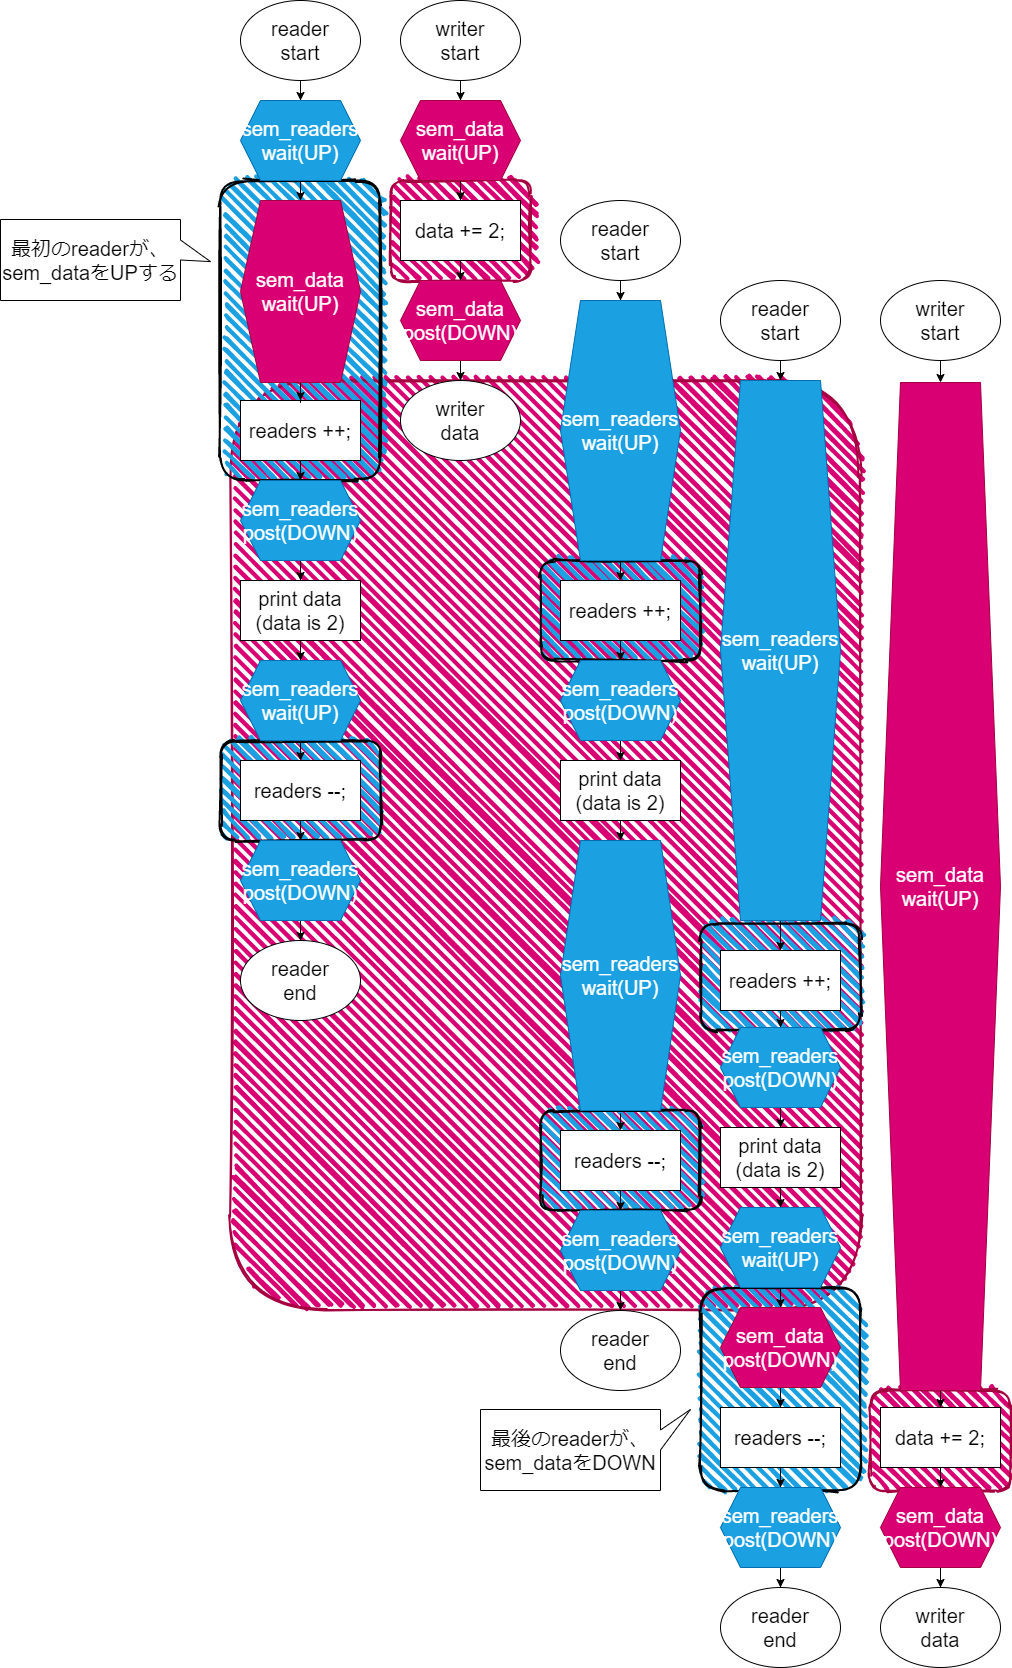
\includegraphics[width=15cm]{01.drawio.png}
\end{figure}

実行結果は、以下のようになった。

\begin{lstlisting}[caption={実行結果},label={実行結果}]
  $ gcc -pthread SemWrite.c
  $ ./a.out
  Data writen by the writer0 is 2
  Data writen by the writer2 is 4
  Data writen by the writer1 is 6
  Data writen by the writer3 is 8
  Data read by the reader0 is 8
  Data read by the reader1 is 8
  Data read by the reader3 is 8
  Data read by the reader4 is 8
  Data read by the reader2 is 8
  Data writen by the writer4 is 10
  Data writen by the writer5 is 12
  Data read by the reader5 is 12
  Data writen by the writer6 is 14
  Data read by the reader6 is 14
  Data writen by the writer7 is 16
  Data read by the reader7 is 16
  Data read by the reader8 is 16
  Data writen by the writer9 is 18
  Data read by the reader9 is 18
  Data writen by the writer8 is 20
\end{lstlisting}

\section{問題2}
すべての哲学者が同時にステップ1を実行すると、誰もステップ2に進むことができない。
全員フォークを置くこともできないので、デッドロックになる。

\subsection{回避するための手順}
以下の手順を、各哲学者が独立して実行する。

\begin{enumerate}
  \item 両隣の哲学者が手を挙げていなければ、手を挙げることができる(同時に挙げたときは、左の哲学者が手を挙げていたら下げる)
  \item 手を挙げることができ、両方のフォークが揃っていれば手順1にしたがって食事する(フォークが揃っていなければ、手を挙げたまま待つ)
\end{enumerate}

この手順で、フォークを双方確保できることが保証できる。
優先度によって、ループして上げ下げが行われる可能性があるが、独立して実行されるので、必ず終息し、デッドロックにはならない。

\end{document}
